In this work, we explore the 
application of multi-instance learning algorithms to the task of partially supervised image segmentation.
Multi-Instance learning is a natural formulation for image classification and has been
successfully applied in this task~\cite{zhou2007multi}. We propose to go a step further and apply
multi-instance learning to the task of object class segmentation in natural
images.  In object class segmentation, the goal is to create a pixel-wise
labeling of an input image into one of several semantic
classes.  Multi-class image segmentation receives much attention in the
computer vision community at the moment. To our knowledge, all previous
methods in the field use strong supervision, meaning manual pixel-wise annotation of
training images. This approach does not
scale to larger datasets, especially if one expects consistency and quality
in the segmentations.

In this work, we investigate the use of multi-instance
learning to obtain multi-class image segmentations using ground truth labeling
only on the image level.
We focus on the multi-class, single label setup, where each image is assigned
one of multiple classes. We formulate multi-class image segmentation as
a multi-instance learning problem by considering each image as a bag of
overlapping candidate segments. 

The standard multi-instance setup is as follows. Let $\mathcal{X}$ be a set of
instances. Then a bag is an element of the power set $2^\mathcal{X}$ and the
task is to learn a function
%\begin{equation}
$f_{MI} \colon 2^\mathcal{X} \rightarrow \{-1,+1\}$
%\end{equation}
from a set of training examples of the form $(X_i,y_i)$ with
bags $X_i \subset \mathcal{X}$ and labels $y_i \in \{-1,+1\}$.  This function
stems from the so-called underlying concept, given by an (unknown) function
$f_{I} \colon \mathcal{X} \rightarrow \{-1,+1\}$, with 
\vspace{-3mm}
\begin{equation}\eqlabel{multi_instance}
f_{MI}(X)= \max_{x \in X} f_{I}(x).
\vspace{-3mm}
\end{equation} 
%In our case, instances are overlapping segments, obtained using constraint
%parametric min-cuts~\cite{carreira2010constrained}.  Each image is a bag
%consisting of hundreds of these segments.
Sometimes, the goal of finding $f_{MI}$ is extended to finding labels not only
on bag-level but also for all the instances within a bag
\cite{liconvex2010,zha2008joint}, i.\ e.\ finding $f_{I}$.\\ 
Even though finding $f_{I}$ is sometimes included in the task statement, there
has been very little work that actually reported accuracy on instance-level. Part
of the reason for this might be that for many of the datasets used in
multi-instance learning no ground truth exists.

We look explicitly at accuracy on instance-level since we are interested in
actually segmenting images, not just classifying them. For multi-class image
segmentation, there are some hand-labeled datasets that provide ground truth
on pixel-level. We use this ground truth to evaluate the performance of our
method. This does not exactly correspond to instance-level ground truth --
since the instances are segments, not pixels -- but relates to it closely.

Since scalability is very important in real-world computer vision
applications, and natural images might need hundreds of segments to
account for all possible object boundaries, we use the efficient
multi-instance kernels~\cite{graetner2002multi}.
Multi-instance kernels are a form of set kernels that transform a kernel
on instance-level to a kernel on bag level.
With $k_I$ denoting a kernel on instances $x,x' \in \mathcal{X}$, we define the
corresponding multi-instance kernel $k_{MI}$ on bags $X,X' \in 2^\mathcal{X}$
as 
\vspace{-2mm}
\begin{equation}
    \eqlabel{mi_kernel}
    k_{MI}(X,X') := \sum_{x \in X, x' \in X'} k^p(x,x'),
\vspace{-2.5mm}
\end{equation}
where $p \in \mathbb{N}$ is a parameter.  As we use the RBF-kernel
$k_{rbf}$ as kernel on $\mathcal{X}$ and powers of RBF-kernels are again
RBF-kernels, we will not consider $p$ in the following.
We normalize the kernel $k_{MI}$ in feature space.

%\begin{equation}
    %k(X,X') := \frac{k_{MI}(X,X')}{\sqrt{k_{MI}(X,X)k_{MI}(X',X')}}.
%\end{equation}
Training an SVM with this kernel produces a bag-level classifier for each class, which we will refer to as MIK.
This procedure is very efficient since the resulting Gram matrix is of size
number of bags, which is much smaller than a Gram matrix of size number of
instances, as is commonly used in the
literature~\cite{andrews2003support,nguyen2010new,zhang2008m3miml}.  Another
advantage over other methods is, that it uses a single convex optimization,
whereas other approaches often use iterative algorithms~\cite{andrews2003support} or need to fit complex
probabilistic models~\cite{zha2008joint}.

While using MIK has many advantages, it produces only an instance-level
classifier. We propose to transform a bag lavel classifier $f_{MI}$ as given by
the SVM and \eqref{mi_kernel} into an instance-level classifier by setting
$f_{I}(x):=f_{MI}(\{x\})$, in other words, by considering each instance as its own
bag. 

To assess the validity of predictions made by $f_{I}$, we transform it
back to an instance-level classifier, using the multi-instance learning
assumption \eqref{multi_instance}. We refer to these instance-based MIK predictions
as MIK-instance. In all experiments, the parameters of the MI-Kernel
and SVM are adjusted using MIK and then used with both MIK and MIK-instance.
This facilitates very fast parameter scans since MIK is very efficient to
compute.

\begin{table}
    \centering
    \vspace{-4mm}
    \begin{tabularx}{0.9\linewidth}{@{\extracolsep{\fill}}lccccccc}
    \toprule
        & SVM-SVR & EMDD & mi-SVM & MI-SVM & MICA & MIK & MIK-instance \\
    \cmidrule(rl){2-8}
    Musk1 & 87.9 &84.9 &  87.4 &  77.9     & 84.3 & 88.0& 88.0 \\
    Musk2 & 85.4 &84.8 &  83.6 &  84.3     & 90.5 & 89.3& 85.2 \\
    \bottomrule
    \end{tabularx}
    \vspace{1mm}
    \caption{Bag level performance of various MIL algorithms on the standard Musk
    datasets. All but MIK provide instance-level labeling. }
    \vspace{-8mm}
    \tablabel{musk-acc}
\end{table}
We compared the performance of MIK, MIK-instance and state-of-the-art MI
methods on the Musk benchmark datasets~\cite{dietterich1997solving}, see
\tabref{musk-acc}. Results were obtained using 10-fold
cross-validation. While the computational complexity of MIK-instance is
very low compared to the other methods, it achieves competitive results.
Using instance-level labels results in a slight loss of accuracy of
MIK-instances, compared to MIK\@. This small degradation of performance is quite surprising, since the model was
not trained to provide any instance-level labels.

For multi-class image segmentation, it is beneficial to have a low witness
rate, i.\ e.\ only a few instances are assumed to be positive in a positive
bag. Since an object might not be very prominent in an image, only a fraction
of segments might correspond to the object.
\tabref{musk-witness} compares the witness rates of MIK-instance,
miSVM~\cite{andrews2003support} and SVR-SVM~\cite{liconvex2010} on the Musk
datasets. MIK-instance is able to achieve similar accuracy
with much less witnesses than the other methods.  Note that Musk1 consists of
very small bags while Musk2 contains significantly larger bags, more similar to the
image/segment setup.
\begin{table}
    \centering
    \vspace{-6mm}
    \begin{tabularx}{.8\linewidth}{@{\extracolsep{\fill}}lcccc}
    \toprule
    & \multicolumn2c{Musk1}  & \multicolumn2c{Musk2}  \\
                &accuracy & witness-rate & accuracy & witness-rate  \\
    \cmidrule(rl){2-3}
    \cmidrule(rl){4-5}
    mi-SVM      & 87.4          & 100\%               &  83.6          & 83.9\%\\
    SVM-SVR     & 87.9          & 100\%               &  85.4          & 89.5\%\\
    MIK-instance& 88.0          & 99\%                &  85.2          & 62.3\%\\
    \bottomrule
    \end{tabularx}
    \vspace{1mm}
    \caption{MIL algorithms and the empirical witness rates of the
    classifiers.}
    \vspace{-10mm}
    \tablabel{musk-witness}
\end{table}
%The MIK-instance method can be extended to the multi-class setup using a
%straight-forward 1-vs-all strategy.
We evaluate the performance of the proposed algorithm for image class
segmentation on the challenging Graz-02 dataset.
This dataset contains 1096 images of three object classes, bike, car and person.
Each image may contain multiple instances of the same class.
From each image, we extract overlapping object-like segments using constraint
parametric min cuts (CPMC,\cite{carreira2010constrained}). We use the top 200 ranked segments and discard the
rest.
Each segment is described using SIFT~\cite{lowe2004distinctive} and
ColorSIFT~\cite{van2009evaluating} features, from which we compute bag of
visual word histograms as well as histograms of oriented
gradients~\cite{dalal2005histograms}. We construct one MI-Kernel per
feature which are combined using multiple kernel learning.
We adjusted parameters on a hold-out validation set and used the
training and test sets as given by the dataset.
It is straight-forward to extend the binary MIK method to the multi-class
setting using a one-vs-all strategy.
We train one MKL-SVM per class using MIK and predict class labels on segment level
using MIK-instance. If at least one SVM classifies a segment as positive,
it is associated with the most confident class. Otherwise it is assigned
``background'' or no class.
This yields a classification of each segment into one of car, bike, person
or background. We merge segments into pixel-level class labels by setting
the label $y_x$ of a pixel $x$ according to
\vspace{-3mm}
\begin{equation}
    y_x = \text{argmax}_{y \in Y} \frac{\#\{S_i | p \in S_i \land y_{S_i}=y \}}{
    \#\{S_i | p \in S_i \}},
\vspace{-3mm}
\end{equation}
where $Y= \{$car, bike, person$ \}$, $S_i$ enumerates all segments within an
image and $y_{S_i}$ is the label of segment $S_i$. In words: each pixel is
assigned the class with the highest ratio of class segments vs non-class
segments containing it.

\begin{table}
    \centering
    \vspace{-6mm}
    \begin{tabularx}{0.8\textwidth}{lRRR}
    \toprule
                & car & bike & person \\
    \cmidrule(l){2-2}
    \cmidrule(l){3-3}
    \cmidrule(l){4-4}
        Pixel-level accuracy&   19.1\%&  27.7\%&  24.6\% \\
    \bottomrule
    \end{tabularx}
    \vspace{1mm}
    \caption{Pixel-level accuracy on the Graz-02 dataset.}
    \vspace{-8mm}
    \tablabel{graz}
\end{table}
If the ratio $\frac{\#\{S_i | p \in S_i \land y(S_i)=y \}}{\#\{S_i | p \in S_i \}}$ 
is smaller than $0.5$ for all labels, i.\ e.\ for all labels there are more
non-class segments than class segments at a given pixel, the pixel
is assigned to the background.
Per-class pixel accuracies are reported in \tabref{graz}, some qualitiative results are shown in \figref{results}. The overall
accuracy on images labels, which is the task that was actually trained, is $87\%$.
While the performance of our multiple-instance based approach is far
from current methods that use pixel-level annotations, whose pixel-level accuracy is around $70\%$~\cite{fulkerson2009class} on pixel-level,
it can serve as a baseline for research on weakly supervised methods for image segmentation..
\begin{figure}[tbp]
	\begin{center}
        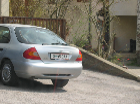
\includegraphics[width=28mm]{images/car1_img.png}\hspace*{0.7ex}
        
\includegraphics[width=28mm]{images/car1_gt.png}\hspace*{0.7ex}
        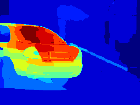
\includegraphics[width=28mm]{images/car1_pos.png}\hspace*{0.7ex}
        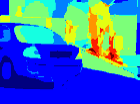
\includegraphics[width=28mm]{images/car1_neg.png}\hspace*{0.7ex}\\
        \vspace{1mm}
        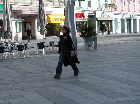
\includegraphics[width=28mm]{images/person1_img.png}\hspace*{0.7ex}
        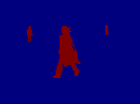
\includegraphics[width=28mm]{images/person1_gt.png}\hspace*{0.7ex}
        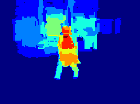
\includegraphics[width=28mm]{images/person1_pos.png}\hspace*{0.7ex}
        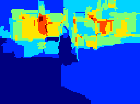
\includegraphics[width=28mm]{images/person1_neg.png}\hspace*{0.7ex}
	\end{center}
        \vspace{-7mm}
        \caption{Qualitative resultson on the Graz-02 dataset. Top: Results on
        category ``car''. Bottom: Results on category ``person''. From left to
        right: original image, ground truth segmentation, segment votes for
        correct class, segment votes against correct class (red many, blue few votes).}
	\figlabel{results}
        \vspace{-7mm}
\end{figure}
